%% -----------------------------------------------------------------------------

\chapter{Evaluation}\label{ch:evaluation}
\glsresetall % Resets all acronyms to not used

In this chapter, the proposed technique for detecting sender MAC addresses during collisions is evaluated using several simulations as well as experiments on WARP software-defined radios.

Possible questions and problems include the fact, that with higher \glspl{MCS}, there could be not enough samples to correlate the rather short 6 byte MAC address. Another interesting issue is the accuracy of the algorithm with increasing amounts of noise and fading.


%% -----------------------------------------------------------------------------

\section{Frequency-Domain Correlation}\label{sec:freqd-correlation}

During the implementation of the MAC address detection technique, I tried using cross-correlation in the frequency-domain. This means that instead of calculating the similarity between samples, complex symbols are correlated without mapping them into the time-domain. With this approach, the Fourier transform must be applied to the received signal.

It turns out to be at least very difficult, if not impossible, to detect senders in case of a collision with frequency-domain correlation. The reason for that is phase shift due to path delays. When a signal is received with an offset in the time-domain, the constellation is changed in the frequency-domain. This can be shown using the Fourier transform equation:

$$ F(f) = \int_{-\infty}^{\infty} s(t) \cdot e^{-2 \pi i f t} dt $$

Here, $ i $ is the imaginary unit, $ F(f) $ is the Fourier transform at frequency $ f $, and $ s(t) $ is the time-domain signal depending on $ t $. A time offset can now be expressed as $ t + \Delta $. Standard power laws then show that this offset introduces a constant multiplication factor on $ F(f) $, depending on $ \Delta $.

$$ F(f) = \int_{-\infty}^{\infty} s(t + \Delta) \cdot e^{-2 \pi i f \cdot (t + \Delta)} dt = \int_{-\infty}^{\infty} s(t + \Delta) \cdot e^{-2 \pi i f t} \cdot e^{-2 \pi i f \Delta} dt = $$
$$ = e^{-2 \pi i f \Delta} \cdot \int_{-\infty}^{\infty} s(t + \Delta) \cdot e^{-2 \pi i f t} dt $$

Since both $ s(t) $ and $ F(f) $ are complex functions, this multiplication is a rotation, or phase shift, in the complex constellation plane. Furthermore, the rotation is different for different frequencies $ f $.

This leads to a received constellation similar to that shown in figure \ref{fig:freqd-corr}. To create this figure, I applied a Rayleigh channel \cite{NEEDED} to a simulated collision signal, introducing a delay of a few nanoseconds. The signals are modulated with BPSK, so ideally the only constellation points should be $ 1 $ and $ -1 $. However, due to the above described rotation, the constellation is basically a circle.

\begin{figure}[ht]
	\centering
	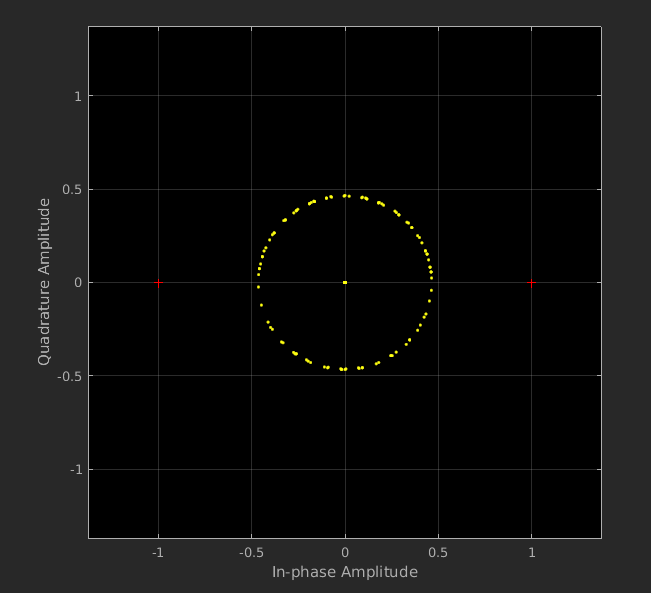
\includegraphics[width=9cm]{gfx/images/freqd-correlation}
	\caption{Cross Correlation of Frequency-Domain Symbols after Channel}
	\label{fig:freqd-corr}
\end{figure}

This kind of path effects is not at all unusual in a IEEE 802.11 transmission. Under normal circumstances, the known preamble is used to calculate the inverted channel matrix of the path effects, as mentioned in section \ref{sec:multipath}.

When receiving a collision, there is however not only one preamble. Instead, the preambles of two different frames, which experienced different path effects, are added together. Since the preambles itself are designed to have a low autocorrelation \cite{NEEDED}, it is not easily possible to separate the two channel effects from each other. Therefore, I can not reverse the phase shift introduced on the OFDM symbols containing the MAC address.

As expected, experiments with cross-correlation in the frequency-domain without channel equalization were unsuccessful. I therefore disregarded this approach.


%% -----------------------------------------------------------------------------

\section{Time-Domain Correlation}


%% -----------------------------------------------------------------------------

\section{Real-World MAC Addresses}\label{sec:real-world-macs}

Note: NIC promiscuitive, otherwise only own and router's MAC will be in the ARP cache!


%% -----------------------------------------------------------------------------

\section{Modulation and Coding Schemes}


%% -----------------------------------------------------------------------------

\section{Scrambler initialization}\label{sec:ex-scrambler}

Note: apparently scrambler init is commonly not chosen at random \cite{NEEDED}


%% -----------------------------------------------------------------------------

\section{Preceeding Data Variations}


%% -----------------------------------------------------------------------------

\section{Channel Models}

Use channel models B, D, and E (most common).


%% -----------------------------------------------------------------------------

\section{WARP Experiments}


%% -----------------------------------------------------------------------------

This is primarily just an example figure to test the matlab2tikz script at this point.\\

\begin{figure}[H]
	\centering
	\setlength\figureheight{5cm}
	\setlength\figurewidth{0.86\textwidth}
	% uncomment the following line to recompile the figure when it changes otherwise a cached version is used
	%\tikzset{external/remake next}
	% This file was created by matlab2tikz.
%
%The latest updates can be retrieved from
%  http://www.mathworks.com/matlabcentral/fileexchange/22022-matlab2tikz-matlab2tikz
%where you can also make suggestions and rate matlab2tikz.
%
\definecolor{mycolor1}{rgb}{0.00000,0.44700,0.74100}%
%
\begin{tikzpicture}[%
font=\footnotesize
]

\begin{axis}[%
width=0.951\figurewidth,
height=\figureheight,
at={(0\figurewidth,0\figureheight)},
scale only axis,
xmin=0,
xmax=7,
xlabel style={font=\color{white!15!black}},
xlabel={MCS},
ymin=0.8,
ymax=1.25,
axis background/.style={fill=white},
title style={font=\bfseries},
title={Time spent on correlating all possible MACs for different MCS},
clip mode=individual,transpose legend,legend columns=2,legend style={at={(0,1)},anchor=north west,draw=black,fill=white,legend cell align=left}
]
\addplot [color=mycolor1, line width=2.0pt, forget plot]
  table[row sep=crcr]{%
0	1.222619\\
1	1.055649\\
2	1.002392\\
3	0.867712\\
4	0.959806\\
5	1.10051\\
6	1.020766\\
7	0.812883\\
};
\end{axis}
\end{tikzpicture}%
	\caption[vary\_mcs-timing-5\_addresses]{Vary MCS: Timing (5 addresses)}
	\label{fig:vary_mcs-timing-5_addresses}
\end{figure}
